\documentclass{bmd2010a}

\usepackage{subfig}

\begin{document}

\begin{flushleft}
{\fontsize{16pt}{20pt}\selectfont%
  Manually Controlled Lane Change Maneuver with 8 Bicycles\\}
\end{flushleft}

%%%%%%%%%%%%%%%% authors %%%%%%%%%%%%%%%
\begin{flushleft}
  {\fontsize{12}{14}{Jason K. Moore, Ronald Hess, Mont Hubbard and Dale L.
  Peterson}\\}
  \textit{Mechanical and Aerospace Engineering\\
          University of California, Davis\\
          One Shields Avenue, Davis, CA 95616, USA\\
          e-mail: jkmoor@ucdavis.edu, rahess@ucdavis.edu, mhubbard@ucdavis.edu,
          dlpeterson@ucdavis.edu
  }\vspace{10pt}\\
\end{flushleft}

\section*{Abstract}

One of the most sought after answers to questions in bicycle dynamics is ``How
will the bicycle handle differently if its phyiscal characteristics are
changed?'' or ``Why do different bicycles handle differently''. The answer to
these questions are not trivial. Many factors play into the picture such as,
but not limited to, the bicycle's dynamics, the rider's dynamics, the rider's
control system, the manuever, the performance criteria and the rider's
subjective opinion of the handling. Of these only the bicycle's dynamics and
the rider's control system are somewhat understoof. Bicycle models have been
shown to predict basic motion through some experientation and much research has
been done in manual control for aircraft pilots.

This work follows in the foot
steps of \cite{Weir1972} and \cite{Lunteren1970} by using the well defined
cross-over model to predict the control action of a rigid person with only the
steering action as an input. We use the physical parameters measured from eight
different bicycles and one rider along with a multi-loop manual control model to simulate a
lane change manuever at three speeds: one below, in and above the linear stable
speed range of the bicycle. Two types of approaches are used. The first is to
tune the control gains for one of the bicycles for good performance. The same
controller is then used for the same manuever for each of the other
bicycle/rider combinations. The overshoot, (other things) are compared and the
bicycles are ranked according to how good or bad the perform under these
criteria. Secondly, a separate controller is tuned for each bicycle/rider for
good performance. We use the same methodology to reach good performance for
each controller design. We then compare peak inputs, gains, and controller
energy? of each bicycle and rank them based on these metrics. I the
relationship between the performance and the phyiscal parameter differences are
analyzed and compared with some anecdotal bicycle lore on how these parameters
changes affect handling.

An ability to predict the handling qualities of bicycles with different
physical characteristics remains an important research issue in the study of
manual control of single-track vehicles. Numerous factors affect bicycle
handling qualities as perceived by the rider, e.g., the dynamics of the bicycle
itself, the dynamics of the rider, the control characteristics of the rider,
and the manner in which the rider quantifies his/her opinion of the bicycle's
handling qualities. The work to be described follows in the footsteps
of~\cite{Lunteren1970} and \cite{Weir1972}, and utilizes a human operator model
discussed in~\cite{Hess2006} as applied to
piloted aircraft control. Figure~\ref{fig:block} is a block diagram representation of the
rider model for roll control of a bicycle, with appropriate sensory modalities
noted. As presented in Fig.~\ref{fig:block}, only three gains and a simple neuromuscular
system model parameterize the rider model. By way of exposition in this brief
abstract, six bicycle models were chosen, five from existing bicycles as
parameterized by the first author, and the sixth the ``benchmark'' bicycle from
~\cite{Meijaard2007}. All models are linear and valid for a forward velocity of 5 m/sec. A
simple 2 m lane change and lane return maneuver was selected for simplicity.
Figure~\ref{fig:path} shows the maneuver paths of the six rider/bicycles, where the bicycle
coordinate shown is associated with the rear wheel contact point. The complete
rider model includes two additional outer-loop closures not shown in
Fig.~\ref{fig:plots} (heading and lateral deviation). In addition, a simple model of rider preview
is included. Figure~\ref{fig:steer} shows the rider steering inputs for the
task. Figure~\ref{fig:handling} shows the ``Handling Qualities Sensitivity
Function'' (HQSFs) for each vehicle.
The magnitude of each of these functions has been shown to correlate well with
handling qualities ratings for aircraft flight control~\cite{Hess2006}. As an example here,
the two functions with the lowest magnitudes in the frequency range of
importance for manual control ($0<\omega$  10 rad/sec) are associated with the two
bicycles models that are either stable or marginally unstable (one root just
into the right-half plane). Finally, Fig.~\ref{fig:bode} shows Bode diagrams for the
rider/bicycle open-loop transfer function for each application, showing that
the rider model follows the dictates of the well-known ``crossover model'' of the
human operator~\cite{McRuer1974}, appropriate for the pure-gain like
$\frac{\phi}{T_\delta}$ dynamics of the
bicycles in question. The final paper will include more bicycle models and
maneuvers and a thorough discussion of applying the HQSF to the prediction of
bicycle handling qualities.
\begin{figure}[tb]
    \centering
    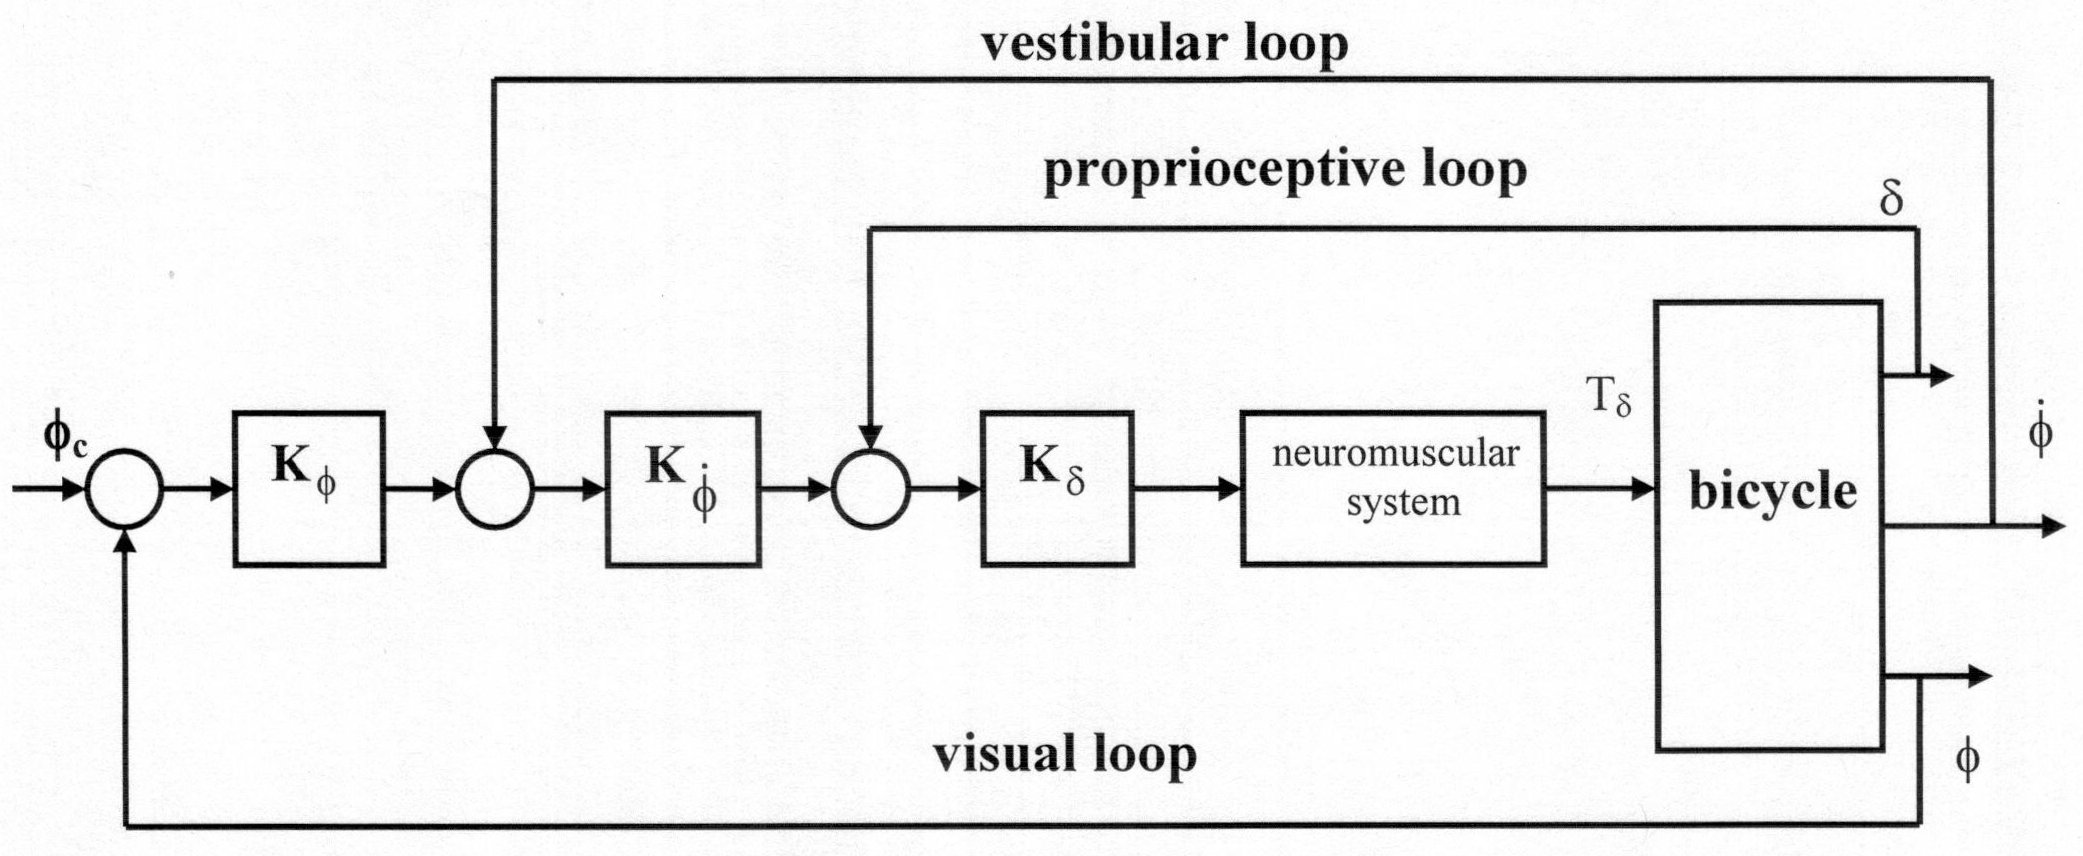
\includegraphics[width=\columnwidth]{block.jpg}
    \caption{Block Diagram of Rider/Bicycle System}
    \label{fig:block}
\end{figure}
\begin{figure}[tb]
    \centering
    \subfloat[Lane Change Performance]{\label{fig:path}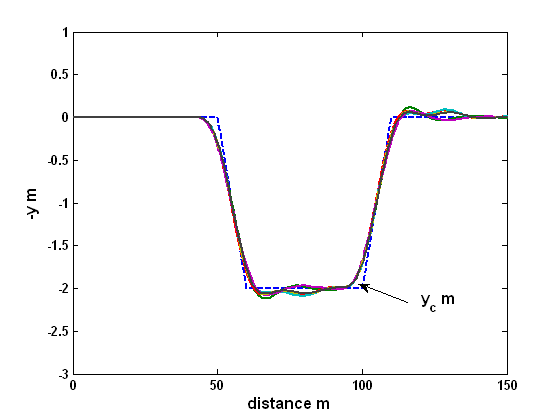
\includegraphics[width=0.5\columnwidth]{path.png}}
    \subfloat[Handling Qualities Sensitivity Functions]{\label{fig:handling}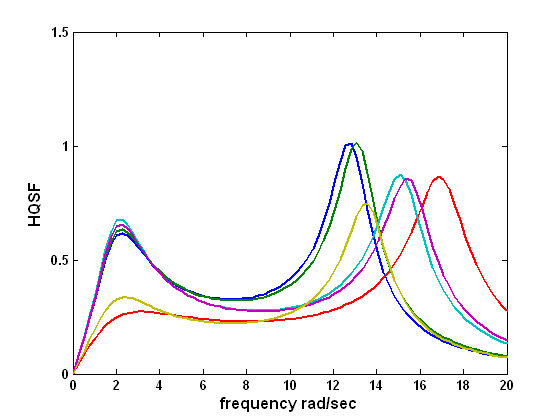
\includegraphics[width=0.5\columnwidth]{handling.png}}

    \subfloat[Rider Steering Inputs]{\label{fig:steer}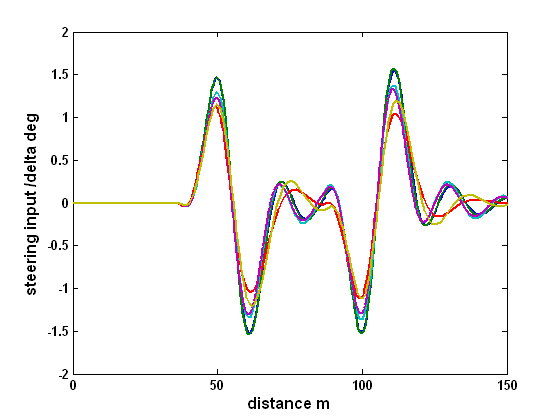
\includegraphics[width=0.5\columnwidth]{steer.png}}
    \subfloat[Bode Diagrams of Rider/Bicycle Open-Loop Transfer
    Functions]{\label{fig:bode}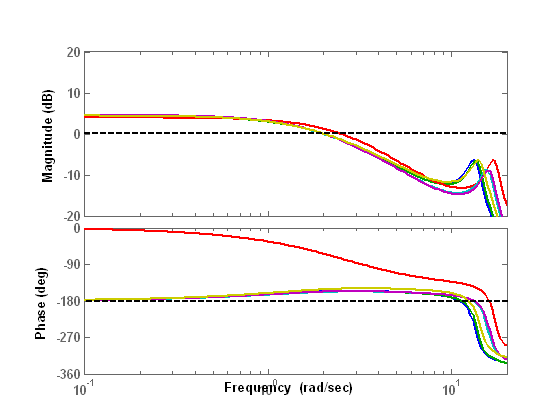
\includegraphics[width=0.5\columnwidth]{bode.png}}
    \caption{Linear simulation results and compartive metrics.}
    \label{fig:plots}
\end{figure}


\bibliographystyle{acm}
\bibliography{bicycle}
\end{document}
